\section{Motivation}\label{sec:intro_motivation}
\begin{marginfigure}[1in]
    \centering
	\begin{subfigure}[b]{\textwidth}
    	\centering
        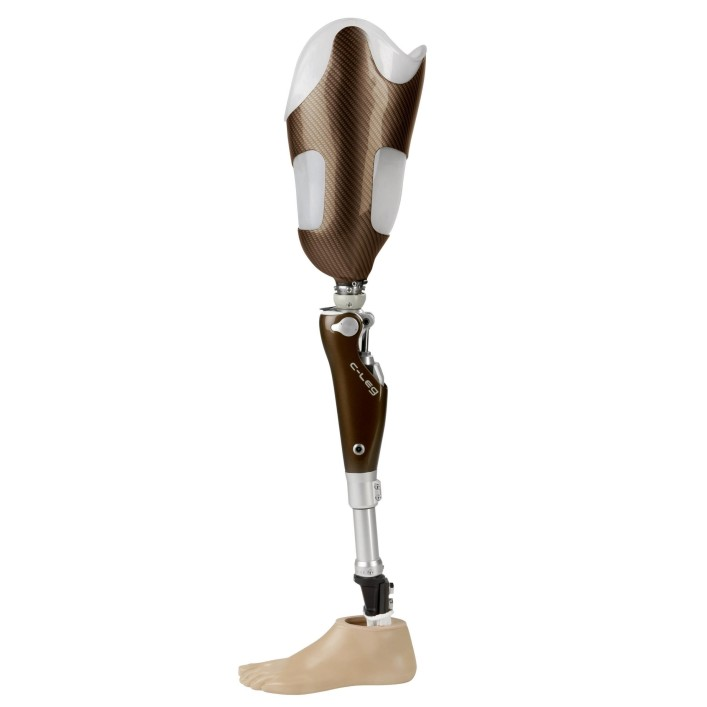
\includegraphics[height=1.5in]{ottobock_cleg}
        \caption{C-Leg™ Knee ©Ottobock}\label{fig:ottobock_cleg}
        \vspace{0.25in}
	\end{subfigure}
	\begin{subfigure}[b]{\textwidth}
    	\centering
        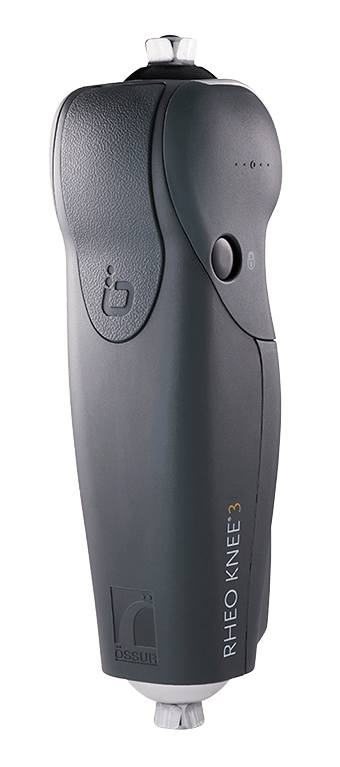
\includegraphics[height=1.5in]{rheo-knee}
        \caption{Rheo™  Knee ©Össur}\label{fig:ossur_rheo}
        \vspace{0.25in}
	\end{subfigure}
	\begin{subfigure}[b]{\textwidth}
    	\centering
        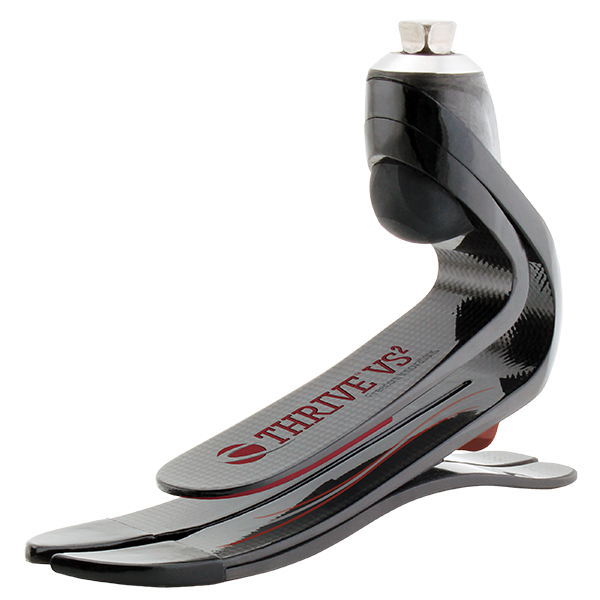
\includegraphics[height=1.5in]{freedom_innov_foot}
        \caption{Thrive™ Foot ©Freedom
        Innovations}\label{fig:freedom_innovations_foot}
	\end{subfigure}
    \caption[Examples of microprocessor-controlled mechanically-passive knee
    prostheses]{Examples of microprocessor-controlled mechanically-passive knee
    prostheses (a,b) and a energy storage and return ankle-foot prosthesis (c).}
\end{marginfigure}
\newthought{Six hundred thousand} lower-limb amputees currently live in the
United States according to recent estimates \citep{ziegler2008estimating}.
People undergo amputations due to a variety of reasons including traumatic
injuries from workplace accidents, traffic collisions, and as casualties of war.
In addition, a large percentage (54\%) suffer from the loss of a limb due to
complications arising from dysvascular disease associated with diabetes.
Consequently, largely due to the expected increase in diabetes in the coming
years, \citet{ziegler2008estimating} estimate that by 2050 the number of
amputees living in the United States will likely double.

Currently, prosthetists often prescribe transfemoral amputees (those with
amputations between the hip and knee joints) an energy storage and return
composite foot such as the Thrive Foot (Freedom Innovations; Irvine, CA;\@
\cref{fig:freedom_innovations_foot}) along with a microprocessor-controlled,
mechanically-passive knee prosthesis. These knee prostheses feature control
algorithms that adjust the knee's resistance in response to kinematic and force
data measured by sensors embedded in the device. Examples of
microprocessor-controlled prosthetic knees include the C-Leg (Otto Bock;
Duderstadt, Germany; \cref{fig:ottobock_cleg}), which has an adjustable
hydraulic damping system, and the Rheo Knee (Össur; Reykjavik, Iceland;
\cref{fig:ossur_rheo}), which achieves variable damping via a magnetorheological
fluid. While \citet{johansson2005clinical} show these microprocessor-controlled
knees can improve amputee gait characteristics by decreasing metabolic energy
consumption and peak hip torque and increasing gait smoothness compared to that
provided by fully-passive knee prosthesis, these prostheses still cannot fully
replicate healthy leg behavior as they are incapable of providing positive net 
power during the gait cycle and are may be limited to providing positive power
only during fixed portions of the gait cycle.

Control of positive power generation is important as positive power is evident
in a number of locomotion tasks. In the knee joint, we see positive power during
level walking \citep{perry2010gait}, walking up stairs
\citep{nadeau2003frontal}, running \citep{buczek1990stance}, and jumping
\citep{hubley1983work}. In addition, active knee flexion and extension muscle
activations have been noted during stumble recovery \citep{eng1994strategies}.
At the ankle joint, passive spring-like prostheses cannot replicate the positive
net work seen in the ankle joint during level ground walking, which is essential
for push-off and forward propulsion \citep{perry2010gait}.

Consequently, lower-limb amputees and especially \emph{transfemoral amputees},
those with above the knee amputations, equipped with mechanically-passive
prostheses suffer from a number of issues including markedly increased energy
consumption~\citep{waters1976energy}, abnormal gait
kinematics~\citep{jaegers1995prosthetic}, and an increased likelihood of
falling~\citep{miller2001prevalence}. Specifically, large percentages of
transfemoral amputees report they are unable to complete tasks such as walking
outside in inclement weather (47.4\%), walking while carrying a load (42.7\%),
walking up or down stairs without a handrail (38.5\%, 37.9\%), walking outside
on uneven terrain (29.5\%), picking up an object from the ground (28.1\%) or
getting up from the floor after a fall (22.8\%) \citep{gauthier1999enabling}.

\begin{figure*}[b]
    \centering
	\begin{subfigure}[b]{0.3\textwidth}
    	\centering
        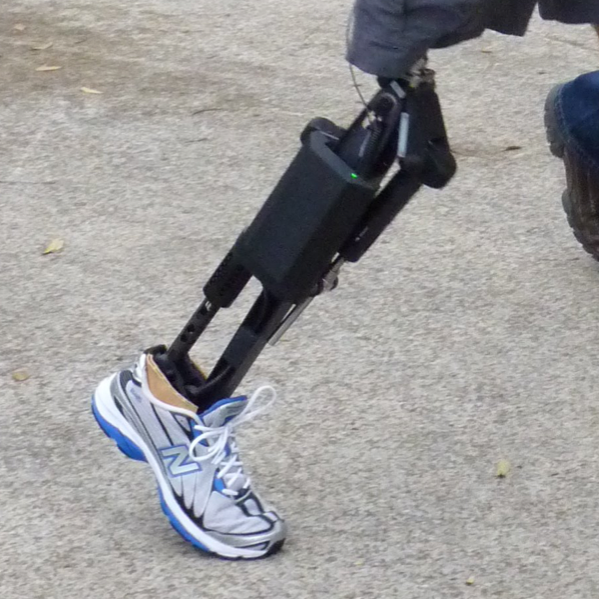
\includegraphics[width=2in]{VU_gen_1}
        \caption{Generation 1}
	\end{subfigure}
	\begin{subfigure}[b]{0.3\textwidth}
    	\centering
        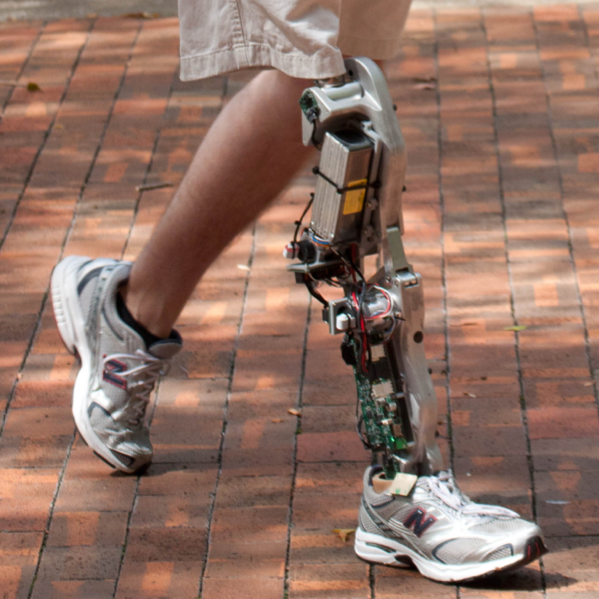
\includegraphics[width=2in]{VU_gen_2}
        \caption{Generation 2}
	\end{subfigure}
	\begin{subfigure}[b]{0.3\textwidth}
    	\centering
        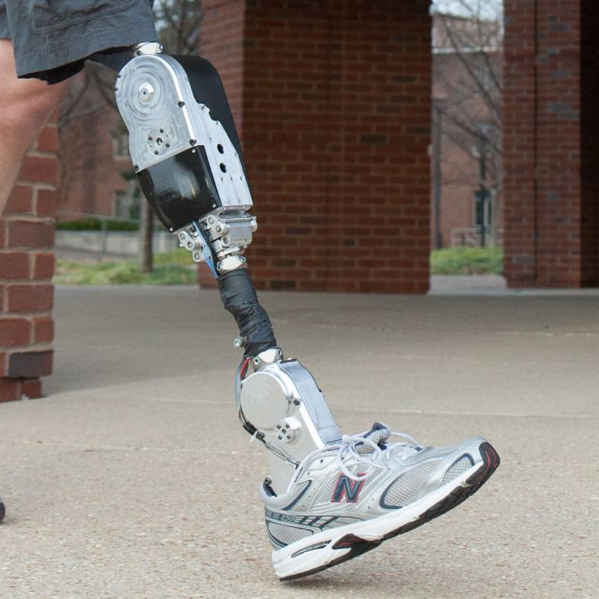
\includegraphics[width=2in]{VU_gen_3}
        \caption{Generation 3}
	\end{subfigure}
    \caption[Vanderbilt University's Robotic Transfemoral Prostheses]{Vanderbilt
    University's Robotic Transfemoral Prostheses. Images courtesy of Michael
    Goldfarb.\vspace{0.1in}}\label{fig:vanderbilt_prostheses_intro}
\end{figure*}

To help remedy this situation, in the past decade academic research groups and
companies have developed robotic powered knee and ankle prostheses for
lower-limb amputees.  These prostheses feature actuators at the knee and/or
ankle that, if controlled correctly, could potentially restore the kinetics,
kinematics, and reactions of the healthy human leg. Notable examples include
three generations of transfemoral prostheses developed by Vanderbilt
University~(\cref{fig:vanderbilt_prostheses_intro}) \citep{sup2009preliminary,
lawson2013control, lawson2014robotic} and the BiOM powered
ankle~(\cref{fig:biom_ankle}) \citep{herr2012bionic}. These powered prostheses
have helped amputees walk on level ground more naturally and efficiently, as
well as walk up stairs and slopes \citep{sup2011upslope, lawson2013control}, run
\citep{huff2012running, shultz2015running}, perform sit-to-stand
\citep{varol2009powered}, and dance \citep{rouse2015design}. These results
illustrate the benefits of powered prostheses as many of these tasks require
positive joint power and thus would be difficult to perform with
mechanically-passive prostheses.

\begin{marginfigure}
    \centering
    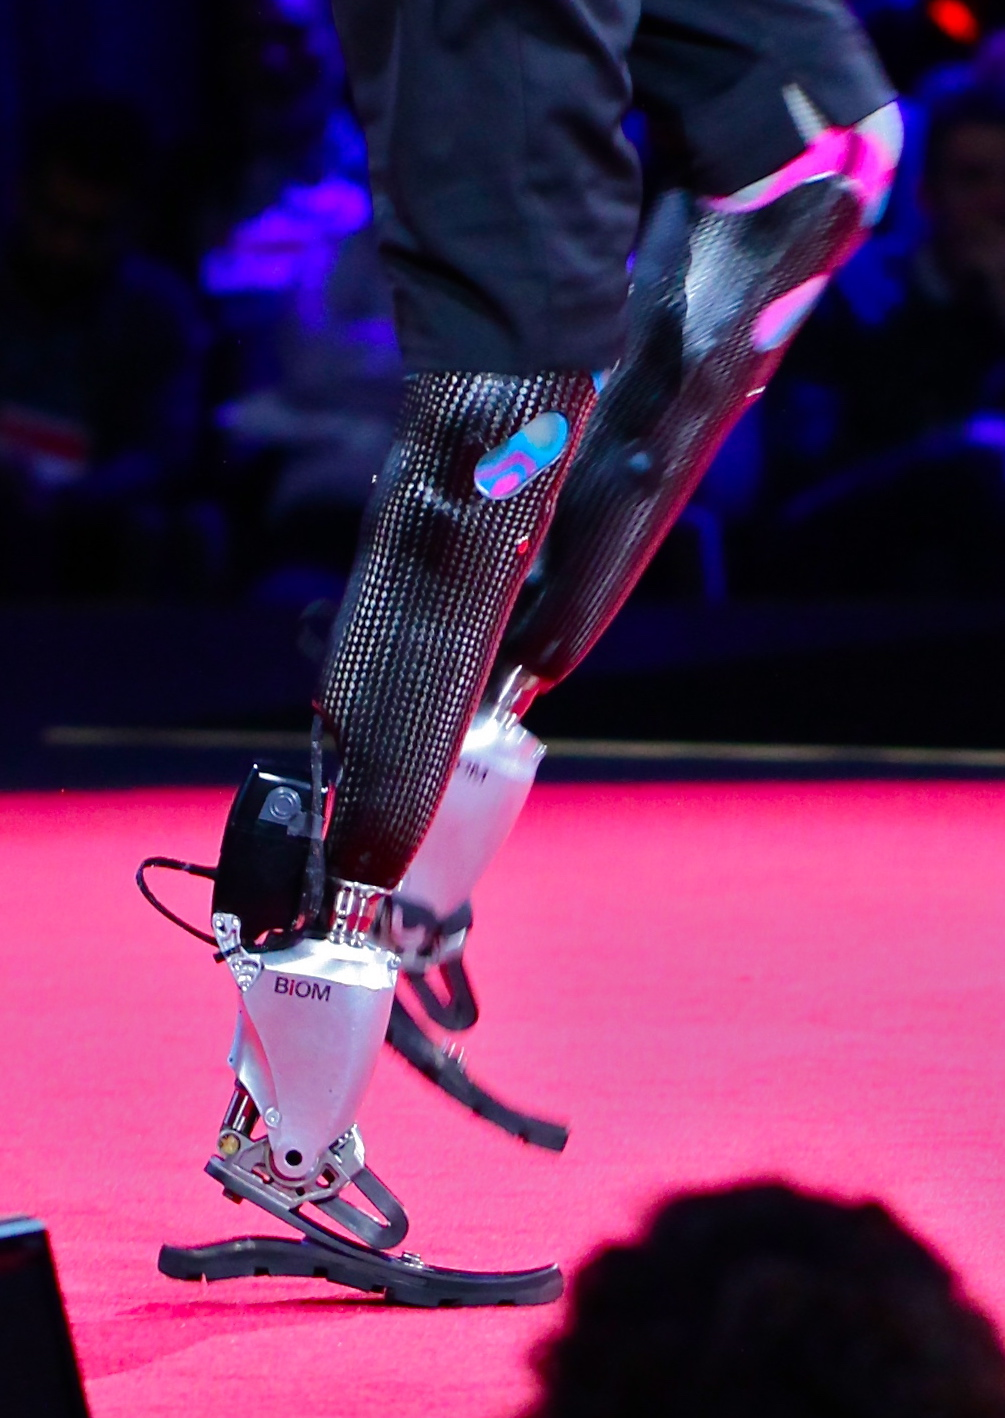
\includegraphics[width=\linewidth]{biom_prosthesis}
    \caption[BiOM Robotic Ankle Prosthesis]{BiOM Robotic Ankle Prosthesis. Photo
    by \href{https://www.flickr.com/photos/jurvetson/13480667874/}{Steve
    Jurvetson}, \href{http://creativecommons.org/licenses/by/2.0}{CC BY 2.0},
    \href{https://commons.wikimedia.org/w/index.php?curid=32568854}{Link}
    (cropped from original).}\label{fig:biom_ankle}
\end{marginfigure}
